\subsection{Human Unit Testing}
\only<presentation>{
\plain{\centerline{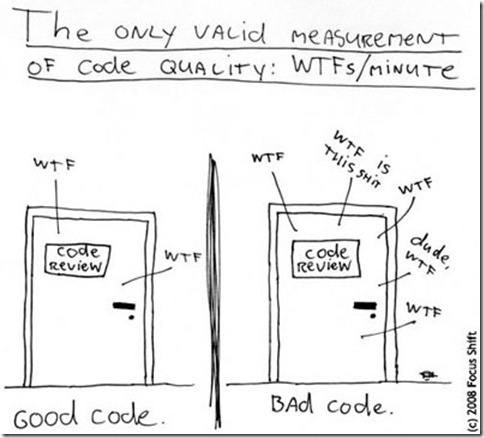
\includegraphics[height=.98\textheight]{content/chapter_testing/testing_intro/wtfs-minute}}}
}
\only<article>{\plain{\centerline{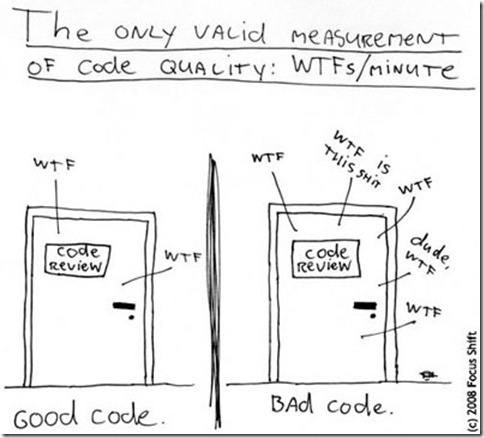
\includegraphics[width=\textwidth]{content/chapter_testing/testing_intro/wtfs-minute}}}\addtocounter{slidenumber}{1}}
\begin{Frame}{Human Unit Testing}
  \begin{itemize}
    \item Reading or visual inspection of a program by a\\
      \alert{team of people} (3-4 persons)
    \item Team includes other people than the programmer(s)
    \item Preparatory work \& conference
    \item Objective: find errors, but not solutions to the errors
    \item Two main techniques: \alert{inspections} and \alert{walkthroughs}
  \end{itemize}
\end{Frame}

\begin{Frame}{Terms}
  \inhead{Review} generic term\hfill\vspace{1ex}\linebreak
  \inhead{Manual review} no automation\hfill\vspace{1ex}\linebreak
  \inhead{Code review} review code, test cases, documentation\hfill\vspace{1ex}\linebreak
  \inhead{Technical review} review requirement documents, diagrams\hfill\vspace{1ex}\linebreak
  \inhead{Peer review} author and colleagues\hfill\vspace{1ex}\linebreak
  \inhead{Walkthrough} review code by playing computer\\
  (sometimes also: information exchange, brainstorming)\hfill\vspace{1ex}\linebreak
  \inhead{Pair programming} review during active development
\end{Frame}

\subsubsection*{Code Inspections}

\begin{Frame}{Code Inspections}
  \begin{itemize}
    \item A set of procedures and error-detection techniques for code reading
    \item Lots of literature on procedures, forms to be filled etc. (Perry, 2000)
    \item Disagreement with respect to whether a group meeting is necessary
    \item For group meeting (Myers, 1979), typically four people: a \alert{moderator}, the \alert{programmer},
    the \alert{program's designer} and a \alert{test specialist}
  \end{itemize}
\end{Frame}

\begin{Frame}{Typical Procedure for Code Inspections}
  \begin{itemize}
    \item The moderator distributes program and specification in advance
    to the other participants
    \item The programmer narrates the logic of the program (helps programmer to find errors)
    \item The program is analyzed with respect to a checklist of errors
    \item The programmer receives a list of the errors found, which is analyzed
    and used to refine the error checklist
    \item Advised length: 90--120 minutes
    \item About 150 lines per hour
  \end{itemize}
\end{Frame}

\begin{Frame}{An Error Checklist}
  \begin{itemize}
    \item sublist of the original list in (Myers, 1979)
    \item Progress in compiler and language design has made many items
    of the original list obsolete.
    \item List divided into \alert{data reference}, \alert{data declaration},
    \alert{computation}, \alert{comparison}, \alert{control-flow},
    \alert{interfaces}, and \alert{input/output} errors.
  \end{itemize}
\end{Frame}

\begin{Frame}{An Error Checklist}{Data Reference}
  \begin{itemize}
    \item Uninitialized variables used?
    \item Array indices within bounds?
    \item String limits exceeded?
    \item Dangling references?
    \item Correct types when aliasing?
    \item Off-by-one errors in indexing or subscripting operations?
  \end{itemize}
\end{Frame}

\begin{Frame}{An Error Checklist}{Data Declaration}
  \begin{itemize}
    \item All variables initialized?
    \item If not, default values understood?
    \item Arrays and strings initialized properly?
    \item All variables have the correct types?
    \item Any variables with similar names?
  \end{itemize}
\end{Frame}

\begin{Frame}{An Error Checklist}{Computation Errors}
  \begin{itemize}
    \item Mixed-mode computations (automatic conversions)?
    \item Intermediate result overflow or underflow?
    \item Division by zero?
    \item Operator precedence understood?
    \item Integer divisions correct?
    \item Variable's value outside of meaningful range?
  \end{itemize}
\end{Frame}

\begin{Frame}{An Error Checklist}{Comparison Errors}
  \begin{itemize}
    \item Comparison relationships correct?
    \item Boolean expressions correct?
    \item Operator precedence understood?
    \item Compiler evaluation of Boolean expressions understood?
  \end{itemize}
\end{Frame}

\begin{Frame}{An Error Checklist}{Control-flow Errors}
  \begin{itemize}
    \item Will each loop terminate?
    \item Will program terminate?
    \item Any loop bypasses because of entry conditions?
    \item Off-by-one iterations errors?
    \item Any non-exhaustive decisions?
  \end{itemize}
\end{Frame}

\begin{Frame}{An Error Checklist}{Interface Errors}
  \begin{itemize}
    \item Parameters and arguments match (number and order)?
    \item Number, attributes, and order of arguments to built-in functions correct?
  \end{itemize}
\end{Frame}

\begin{Frame}{An Error Checklist}{Input/ Output Errors}
  \begin{itemize}
    \item Format specification matches I/O statement?
    \item Buffer size matches record size?
    \item Files opened before use?
    \item End-of-file conditions handled?
    \item I/O errors handled?
    \item Any textual errors in output information?
  \end{itemize}
\end{Frame}

\begin{Frame}{An Error Checklist}{Other Checks}
  \begin{itemize}
    \item Any unreferenced variables in cross-reference listing?
    \item Any warning or informational messages?
    \item Input checked for validity?
    \item Missing function?
  \end{itemize}
\end{Frame}

\begin{Frame}[allowframebreaks]{An Error Checklist}{Some (Rather) Obsolete Errors}
  \begin{itemize}
    \item Computing addresses of bit strings? Passing bit-string arguments?
    \item Structure definitions match across procedures?
    \item All variables declared?
    \item Initialization consistent with storage class?
    \item Computations on non-arithmetic variables?
    \item Base-2 inaccuracies?
    \item Comparison and Boolean expressions mixed?
  \end{itemize}
  
  \framebreak

  \begin{itemize}
    \item Comparisons of base-2 fractional values?
    \item Do begin and end statements match?
    \item Number of arguments transmitted to called modules equal to number of parameters?
    \item Attributes of arguments transmitted to called modules equal to attributes of parameters?
    \item Units system of arguments transmitted to called modules equal to units system of parameters?
  \end{itemize}
\end{Frame}

\subsubsection*{Walkthroughs}

\begin{Frame}{Walkthroughs}
  General scheme similar to that of inspections, but:
  \begin{itemize}
    \item A member of the team acts as \alert{tester}.
    \item The tester comes to the meeting with some test cases.
    \item The participants \alert{play computer}, the current state of the program is monitored.
  \end{itemize}
\end{Frame}

\begin{Frame}{Empirical Data on Walkthroughs}
  \begin{itemize}
    \item Several studies available in the literature.
    \item Code distributed to some testers (small groups) in controlled situations.
    \item Code inspection finds between 30 and 50 \% of all errors.
  \end{itemize}
\end{Frame}

\subsubsection*{Social Effects}

\begin{Frame}[fragile]{Social Effects: Knowledge}
  Knowledge spreads through the team
  \begin{itemize}
    \item Experts and juniors share knowledge
    \item Real-time feedback for developers
    \item \alert{Responsibility} for entire project on whole team Maintaining not only depends on author
    \item Developers learn to spot errors and are more cautious New team members get to know the project
    \item Improve teamwork, because learning from each other becomes natural
  \end{itemize}
\end{Frame}

\begin{Frame}{Social Effects: Illusionary Confidence}
  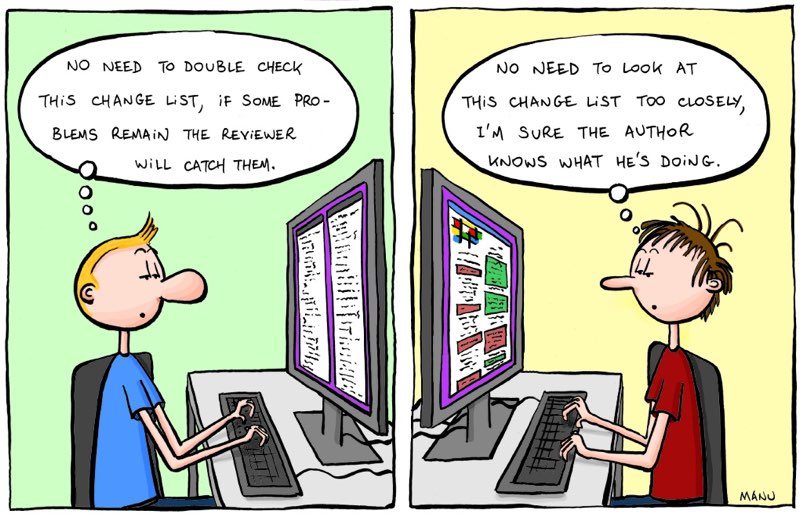
\includegraphics[width=\textwidth]{content/chapter_testing/testing_intro/confidence}

  \xxx

  \source{\href{http://www.bonkersworld.net/code-reviews}{www.bonkersworld.net/code-reviews}, December 1, 2013}
\end{Frame}

\begin{Frame}{Social Effects: Reputation}
  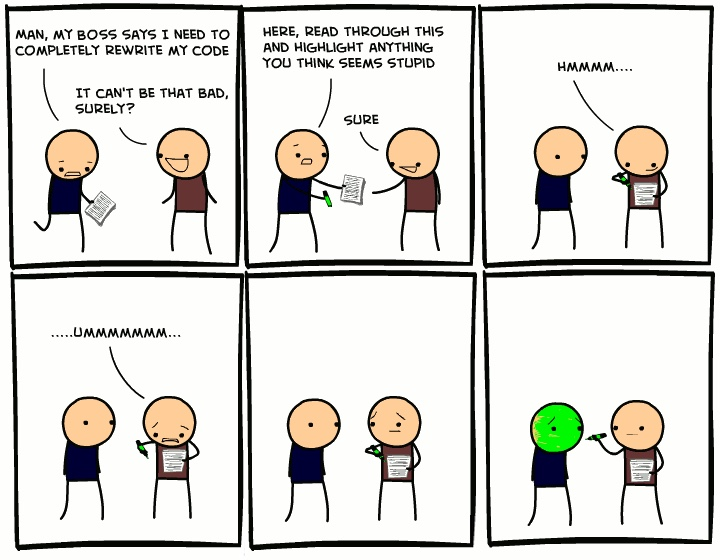
\includegraphics[width=\textwidth]{content/chapter_testing/testing_intro/reputation}

  \source{\href{http://blog.manishchhabra.com/2012/12/code-reviews-should-be-the-universal-rule-of-serious-software-development/}{blog.manishchhabra.com/2012/12/ code-reviews-should-be-the-universal-rule-of-serious-software-development/}, December 1, 2013}
\end{Frame}

\begin{Frame}{Social Effects}{Some Advices for Managers}
  \begin{itemize}
    \item Its about the code, not the person!
    \item Mix the code review team members.
    \item Explain to the team, that you \alert{want} them to find defects.
  \end{itemize}
\end{Frame}

\begin{Frame}{Social Effects}{Some Advices for Reviewers}
  \begin{itemize}
    \item Also point out good things!
    \item Be respectful, and patient.
    \item Everyone makes mistakes, even you.
    \item Learn from others, from their skills and\\
      from their mistakes.
    \item Avoid accusations, ask questions\\
      instead of making statements.
  \end{itemize}

  \xxx

  \source{Improve Quality and Morale: Tips for Managing the Social Effects of Code Review, SmartBear Software,
\href{http://support.smartbear.com/resources/cc/codereviewsocialeffects.pdf}{support.smartbear.com/resources/cc/codereviewsocialeffects.pdf}, June 15, 2014}
\end{Frame}




